\documentclass[12pt,a4paper]{article}
\usepackage[utf8]{inputenc}
\usepackage{amsmath}
\usepackage{listings}
\usepackage{verbatim}
\usepackage{graphicx} 
\oddsidemargin 0cm
\marginparwidth 0cm
\hoffset 0cm
\usepackage{polski}
\begin{document} 
\large
\begin{tabular}{|c|c|c|c|}
\hline
\multicolumn{4}{|l|}{Temat:}\\
\multicolumn{4}{|c|}{Szybka transformata sinusowa}\\
\hline
\multicolumn{1}{|l}{Wykonał:}&\multicolumn{1}{|l}{Wydział:}&\multicolumn{1}{|c}{Kierunek}&\multicolumn{1}{|l|}{Grupa:}\\
Marcin Fabrykowski&FiIS&Inf. Stos.&grupa 3\\
\hline
\end{tabular}
\normalsize
\vspace{2cm}
\begin{enumerate}
\item Wstęp\\
Szybka transformata sinusowa to liniowa i~odwracalna funkcja prowadząca z~$R^N\rightarrow R^N$. Definiuje się ją jako: $$X_k=\sum\limits_{n=0}^{N-1}x_n\sin \left[ \dfrac{\pi}{N+1}(n+1)(k+1)\right],\ k=0,1,2,\dots,N-1$$
\item Wykonanie ćwiczenia\\
Zaczynamy od wygenerowania sygnału okresowego zgodnie ze wzorem:
$$y_0(i)=\sin(\omega\cdot i)+\sin(2\omega\cdot i)+\sin(3\omega\cdot i)$$
przy założeniu że $\omega=2\dfrac{2\pi}{n}$\\
Następnie do naszego sygnału generujemy szum. Szum będzie w~zakresie $a\in(-1,1)$. Generujemy go wykorzystując zmienną losową $$X=\dfrac{rand()}{RAND\_MAX+1.0}$$
$$a=2*X-1$$
Nasz sygnał z~szumem będzie miał postać: $y(i)=y_0(i)+a$.\\
Zapisujemy nasz sygnał do wektora. Długość wektora wynosi $n=2^k$.\\
Następnie wykonujemy szybką transformatę sinusową. Do tego celu używamy funkcji \textbf{sinft} z~biblioteki Numerical Reciples.\\
Wyznaczamy wartość maksymalną, a~następnie zerujemy wartości mniejsze niż 25\% wartości maksymalnej.\\
Wykonujemy odwrotną transformatę sinusową. Wykonuje się ją poprzez ponowne wykorzystanie funkcji \textbf{sinft}, a~następnie pomnożenie wyniku przez $\dfrac{2}{n}$\\
Powyższe zadanie wykonuje program:
\lstinputlisting[language=C++,caption=main.cpp,breakatwhitespace=true,basicstyle=\footnotesize,breaklines=true]{main.cpp}
którego argumentem jest wartość \textit{k}.\\
Wykorzystując skrypty:\\
\lstinputlisting[language=bash,caption=plot.sh,breakatwhitespace=true,basicstyle=\footnotesize,breaklines=true]{plot.sh}
\lstinputlisting[language=bash,caption=plot2.sh,breakatwhitespace=true,basicstyle=\footnotesize,breaklines=true]{plot2.sh}
\lstinputlisting[language=bash,caption=plot3.sh,breakatwhitespace=true,basicstyle=\footnotesize,breaklines=true]{plot3.sh}
wykonujemy wykresy.
\begin{figure}
\caption{k=10, pełny zakres sygnału zaszumionego}
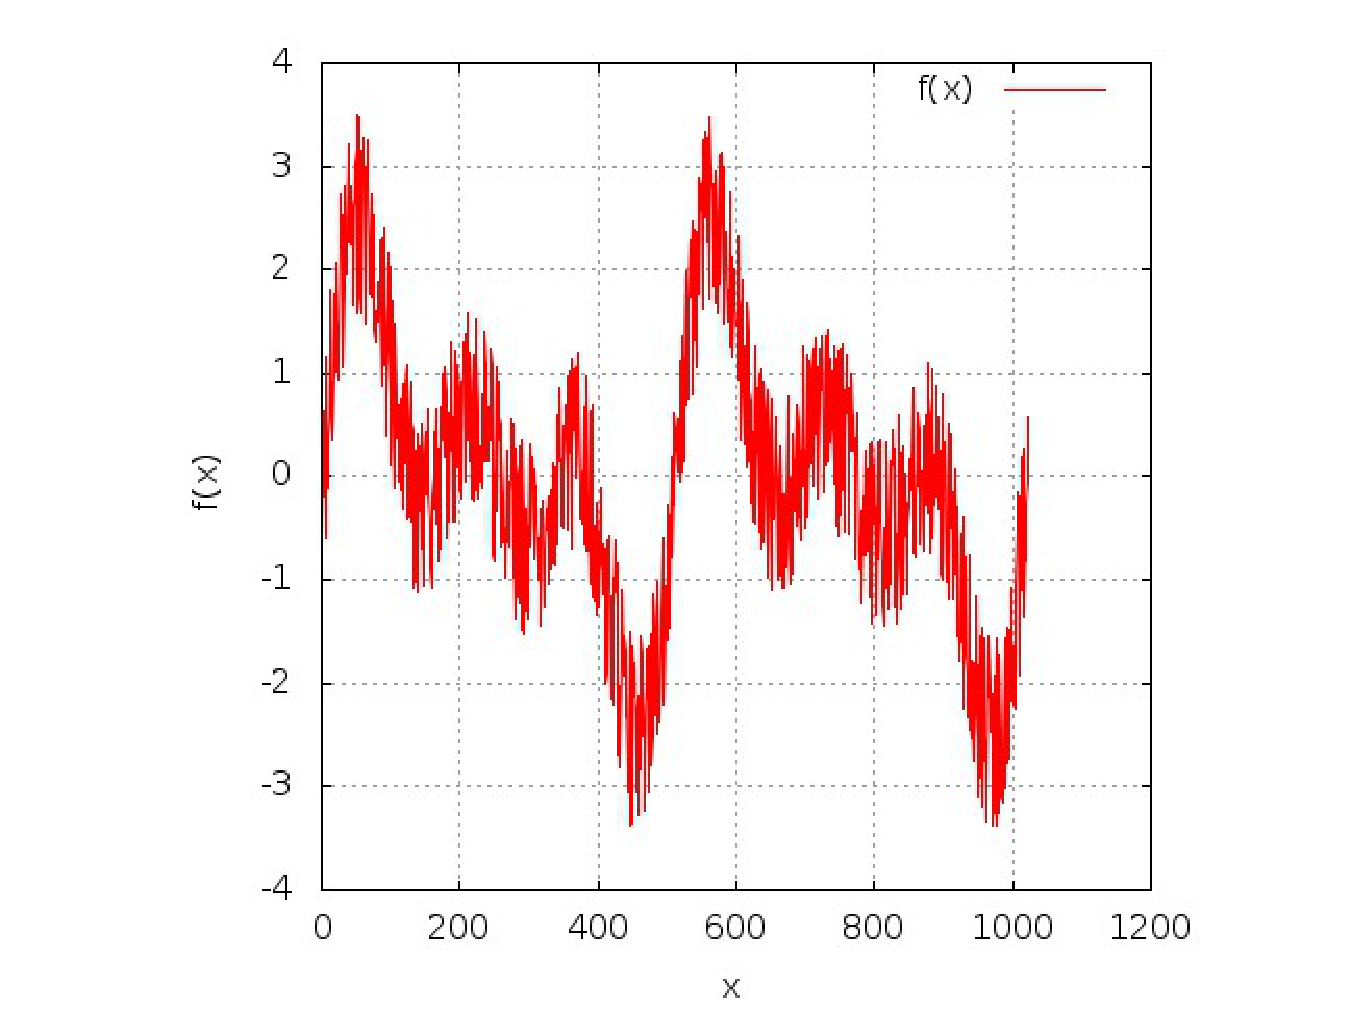
\includegraphics{k_10_1.eps}
\end{figure}
\begin{figure}
\caption{k=10, transformata z~widocznymi pikami}
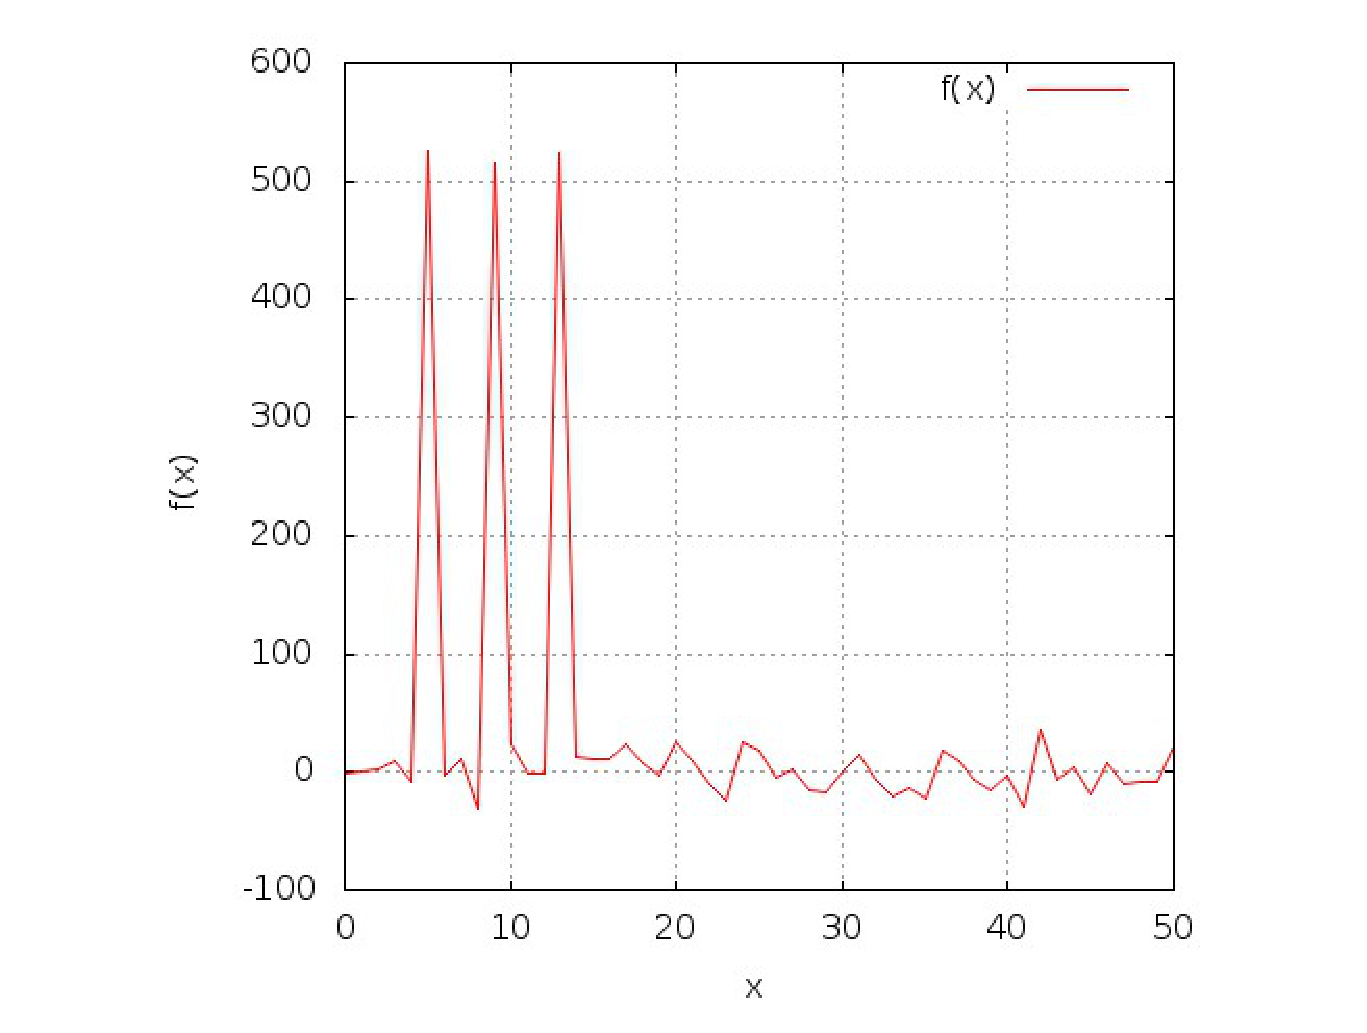
\includegraphics{k_10_2.eps}
\end{figure}
\begin{figure}
\caption{k=10, sygnał niezaszumiony i~odszumiony}
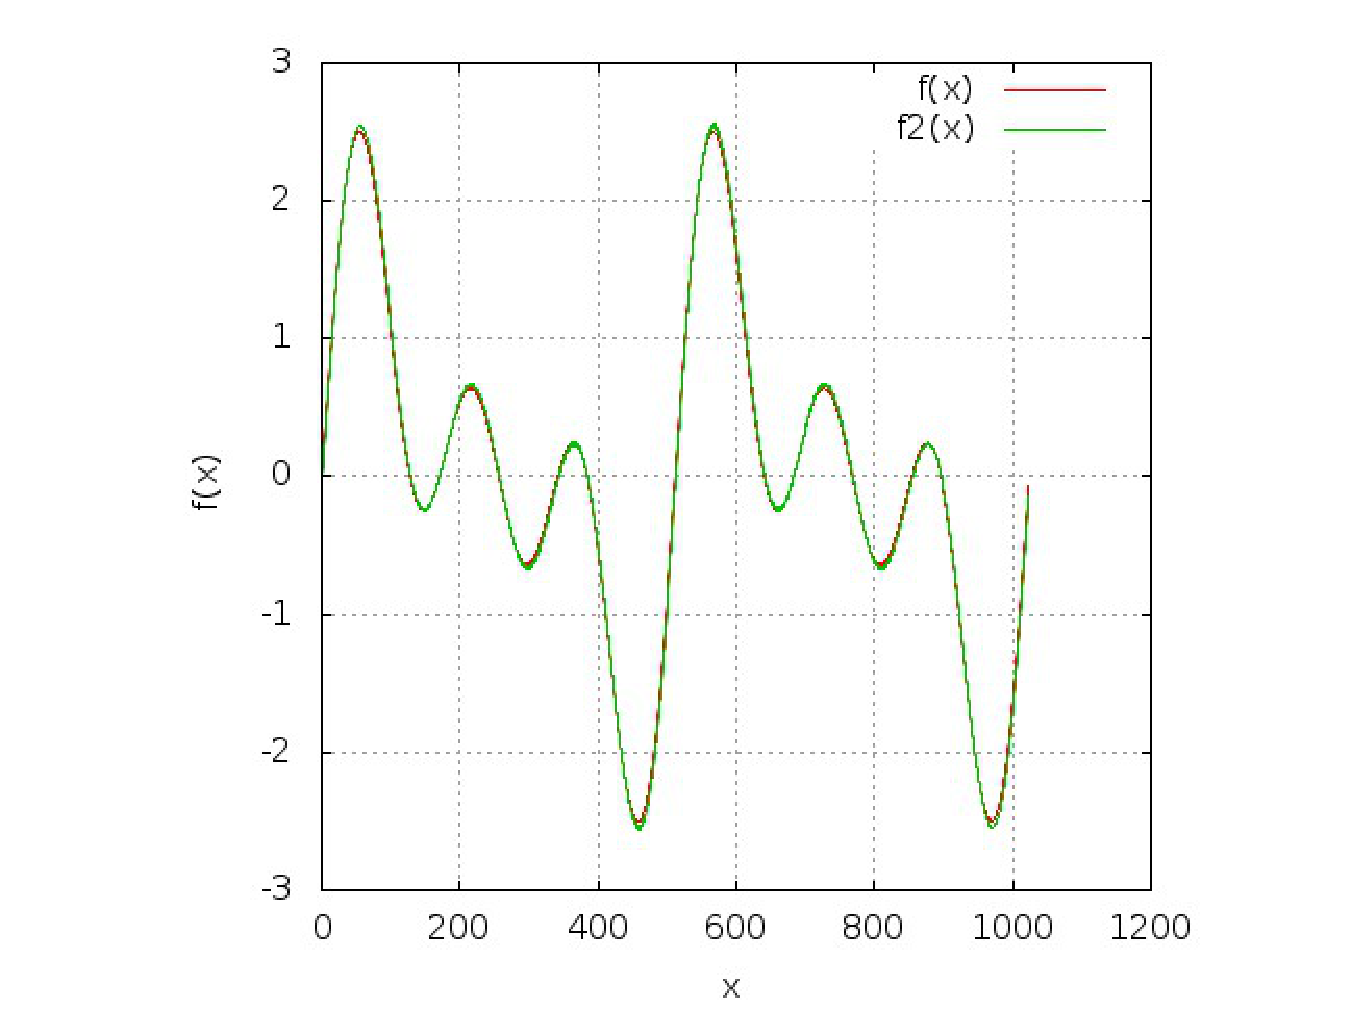
\includegraphics{k_10_3.eps}
\end{figure}
\begin{figure}
\caption{k=10, transformata w~pełnym zakresie}
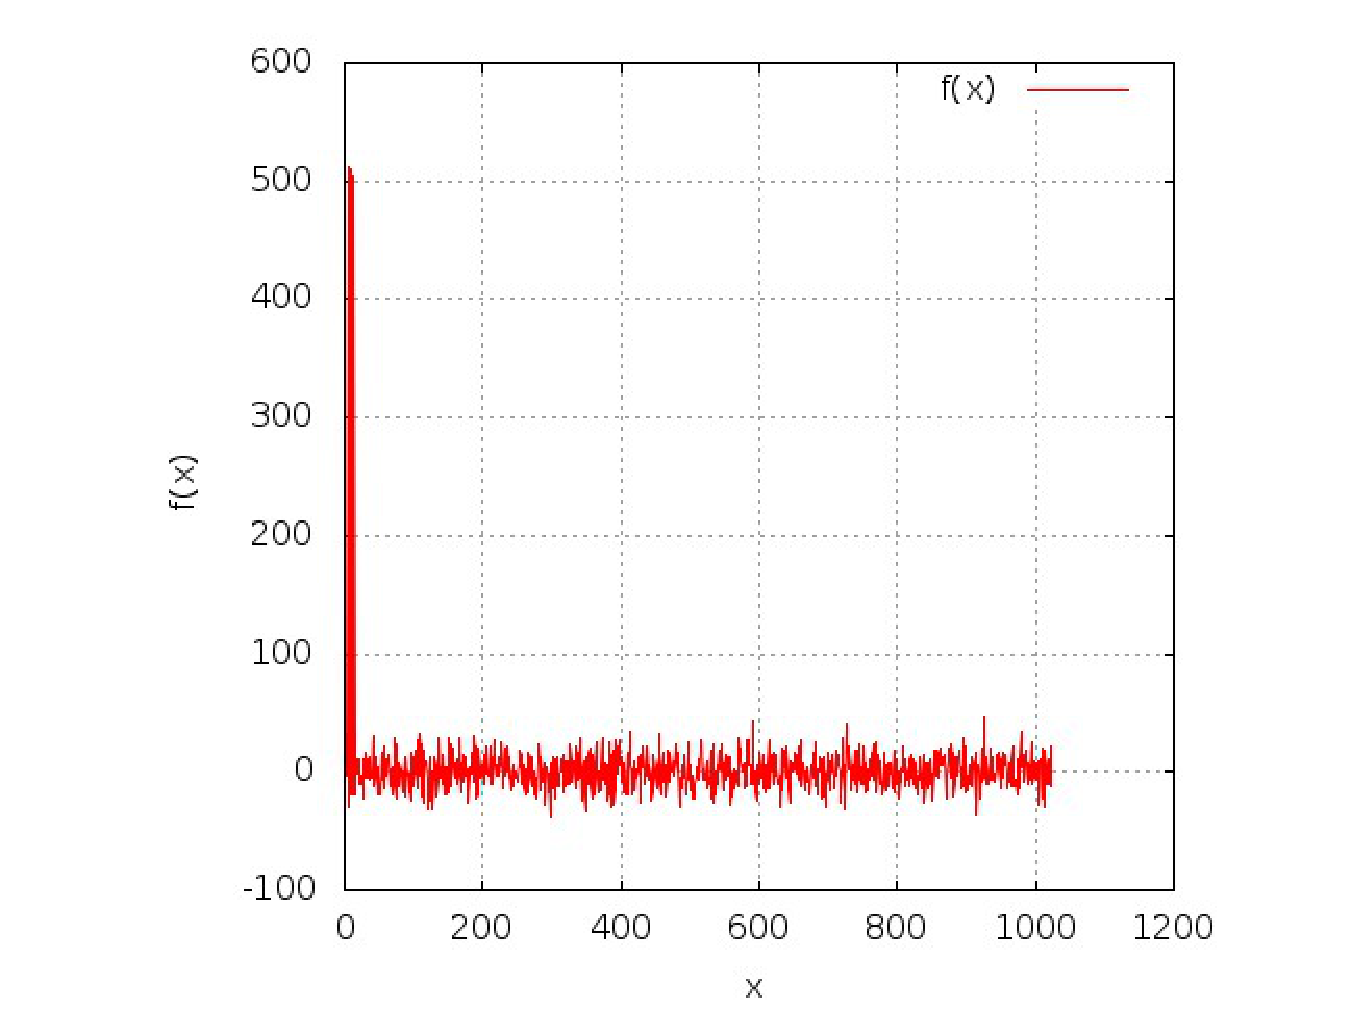
\includegraphics{k_10_4.eps}
\end{figure}
\begin{figure}
\caption{k=8, transformata w~pełnym zakresie}
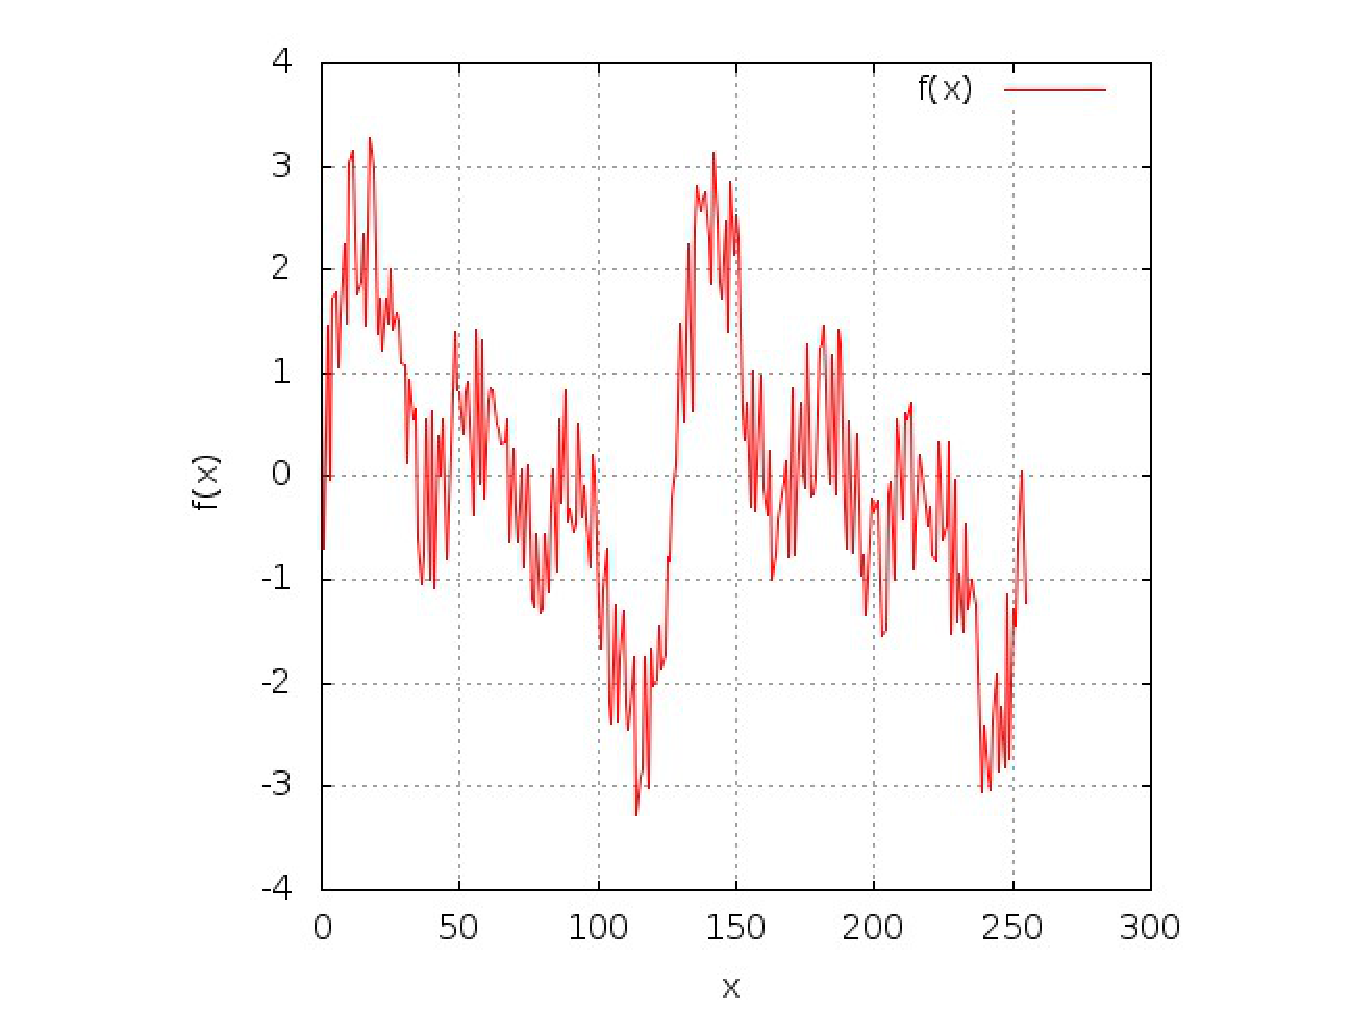
\includegraphics{k_8_1.eps}
\end{figure}
\begin{figure}
\caption{k=8, transformata z~widocznymi pikami}
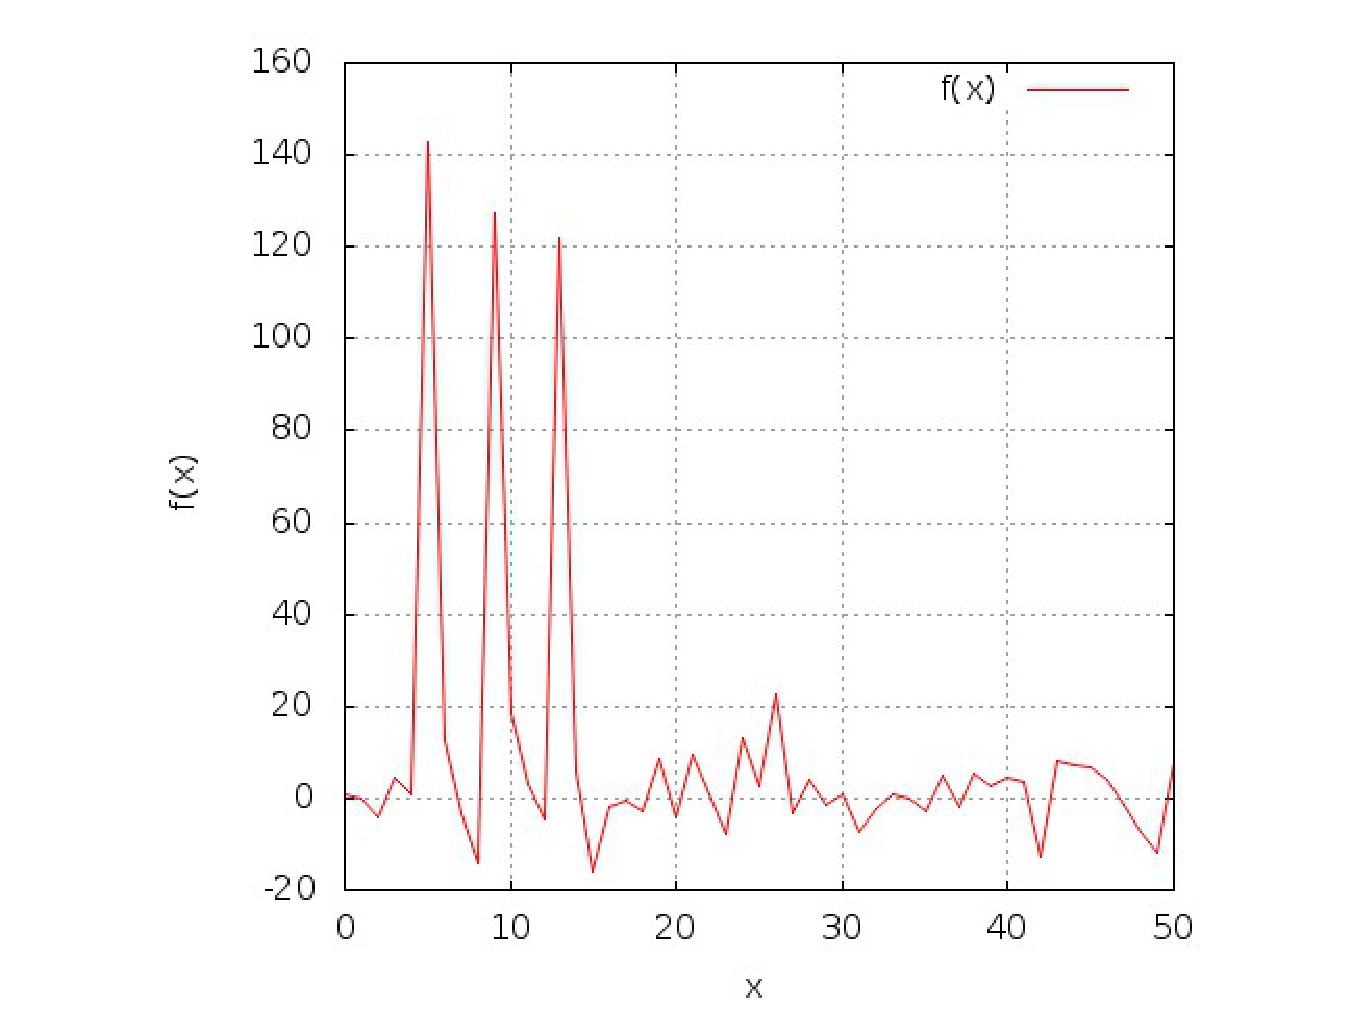
\includegraphics{k_8_2.eps}
\end{figure}
\begin{figure}
\caption{k=8, sygnał niezaszumiony i~odszumiony}
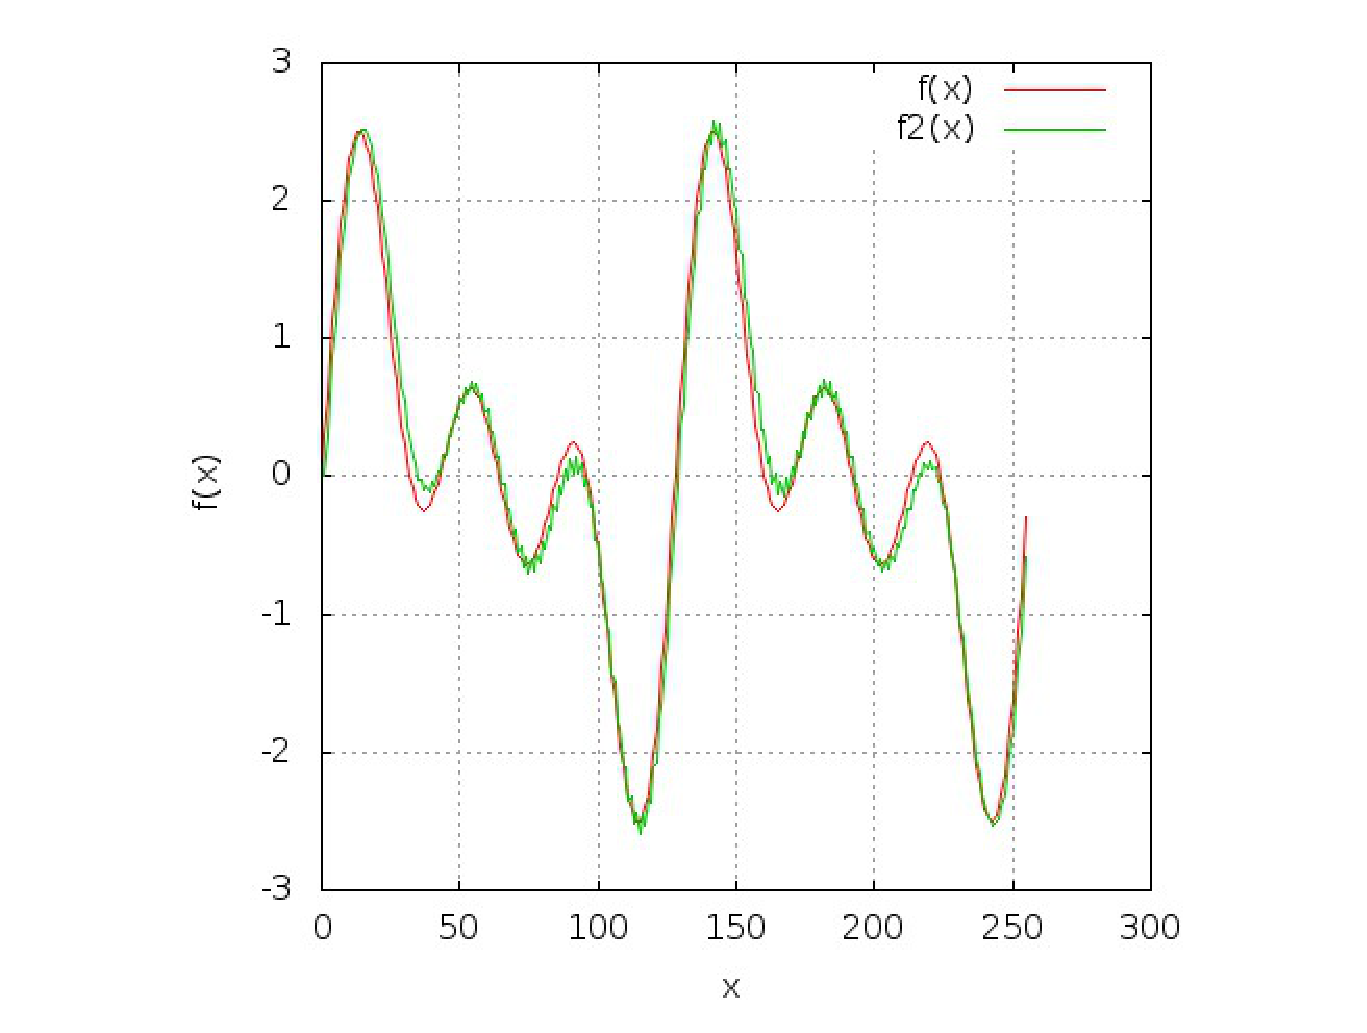
\includegraphics{k_8_3.eps}
\end{figure}
\begin{figure}
\caption{k=6, transformata w~pełnym zakresie}
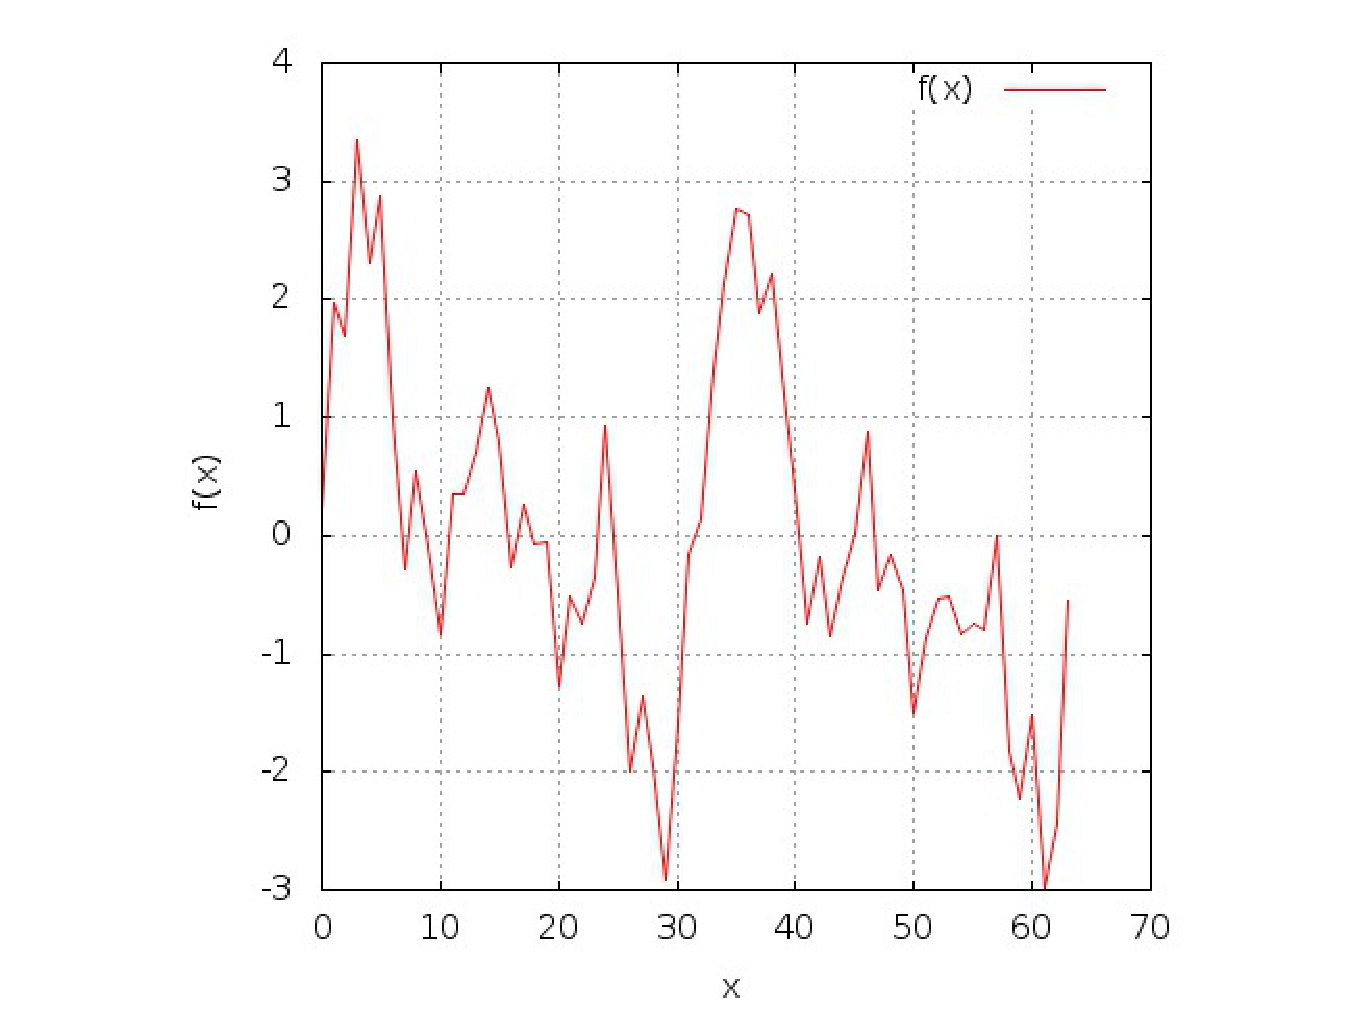
\includegraphics{k_6_1.eps}
\end{figure}
\begin{figure}
\caption{k=6, transformata z~widocznymi pikami}
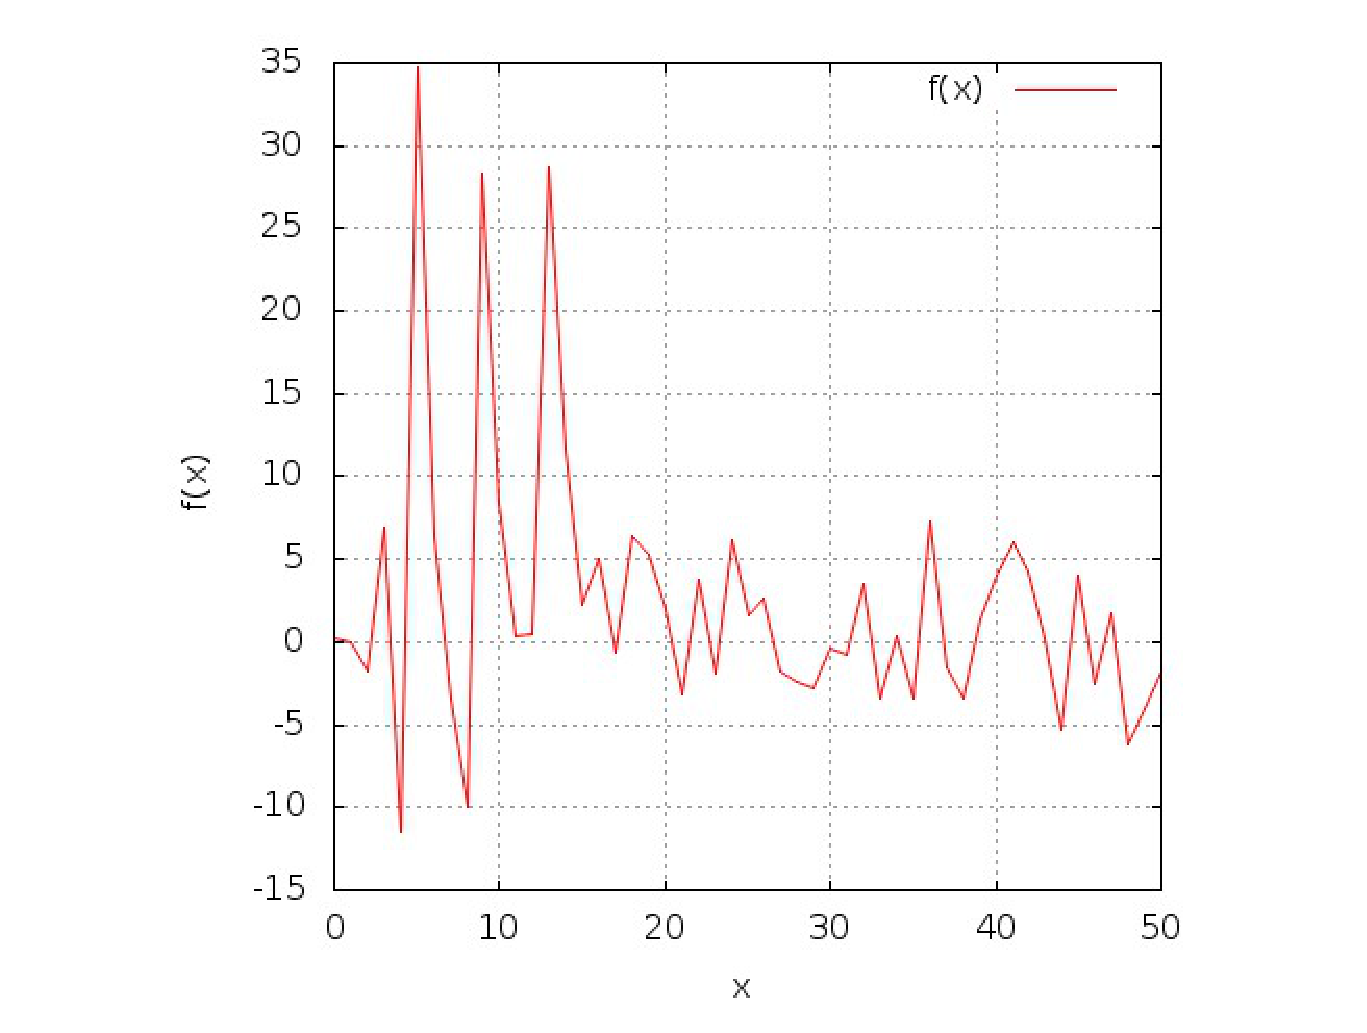
\includegraphics{k_6_2.eps}
\end{figure}
\begin{figure}
\caption{k=6, sygnał niezaszumiony i~odszumiony}
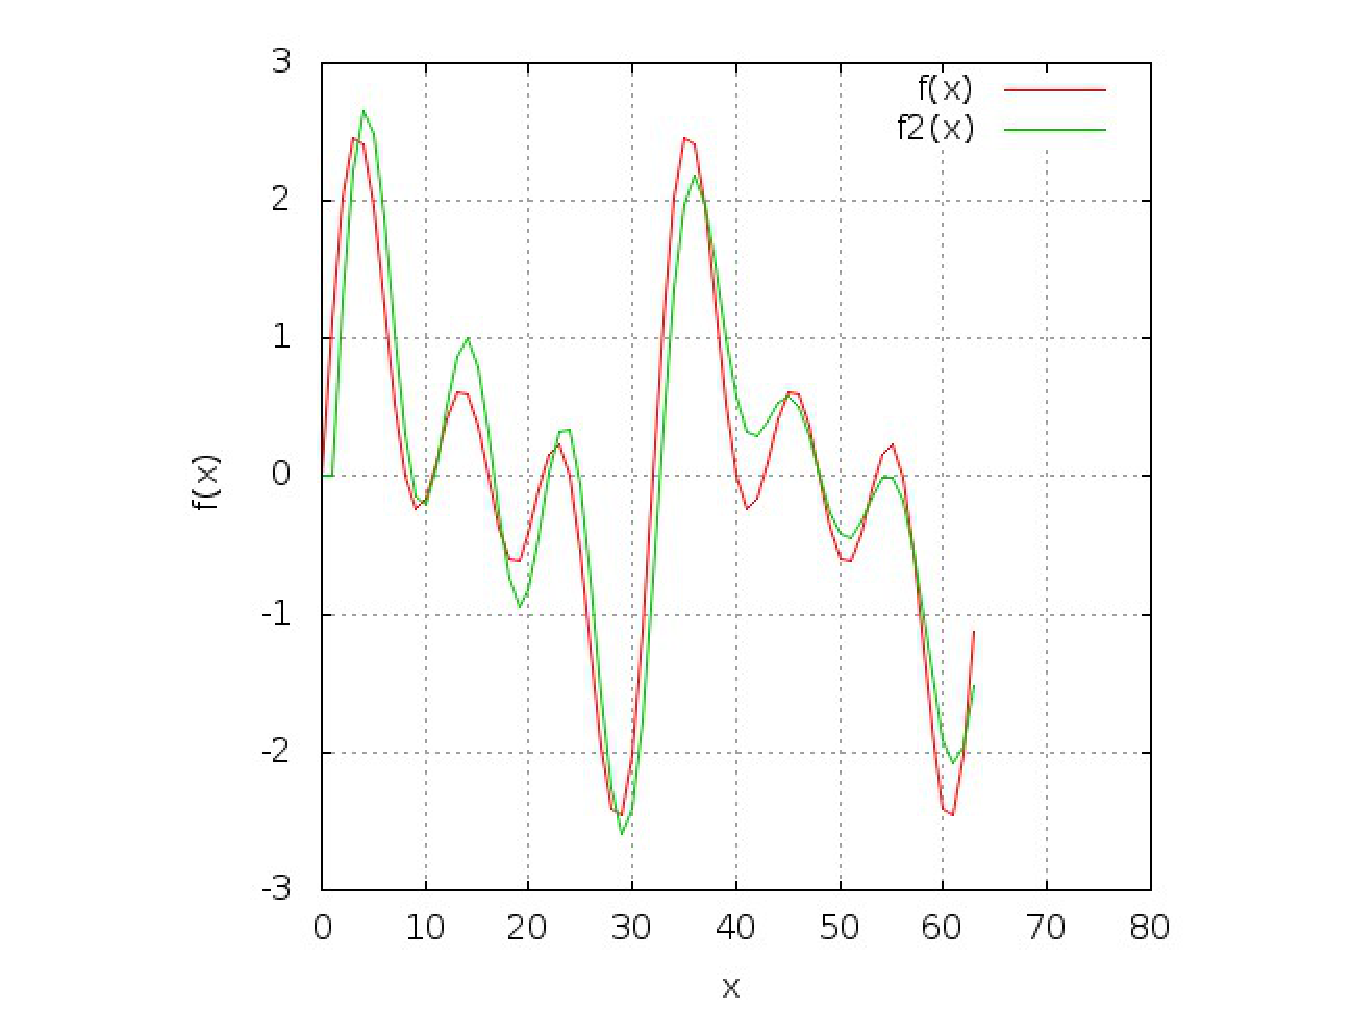
\includegraphics{k_6_3.eps}
\end{figure}
\item Wnioski\\
Jak widać, metoda transformaty sinusowej sprawdza się w~odszumianiu sygnałów. Dokładność ta rośnie wraz z~\textit{k}. Przy $k=10$ widać praktycznie idealne nałożenie się sygnału pierwotnego i~odszumionego. Dla $k=6$ zauważamy pewnie niedokładności jednak ich poziom oceniam jako dopuszczalny.
\end{enumerate}
\end{document}
